\chapter{Complex Numbers: $i^2$ Keep it Real}

\section{The complex number: $i$} \label{apx:complex}
Electromagnetics makes heavy use of complex numbers, which we employ to tell us
about waves.  The representation of the complex quantity $i$ is defined as
\begin{equation}
    i \equiv \sqrt{-1}.
\end{equation}
This leads to the obvious result $i \cdot i = i^2 = -1$.

Perhaps you were taught in a previous math course that roots of negative numbers
was not allowed.  This is only true in that the root of a negative number cannot
produce a value along the real number line.  However, imagine a second number
line orthogonal (independent) of the real number line that does allow for roots
of complex values.  We call the set of numbers that fall along this line
imaginary numbers (Figure~\ref{fig:complex}).
\begin{figure}[hbt]
  \centerline{
    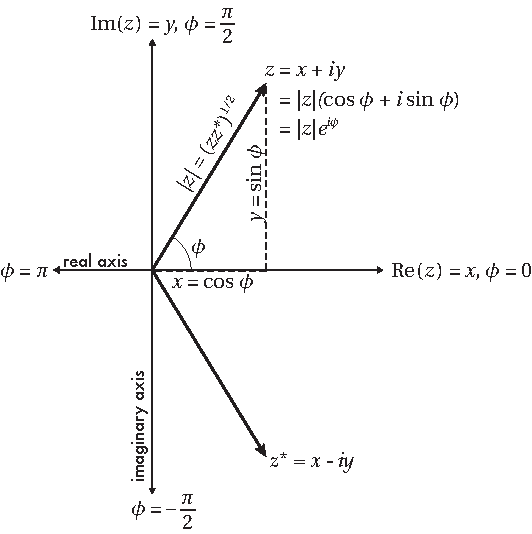
\includegraphics[]{math_primer/figures/complex_plane.eps}
  }
  \caption{Complex plane and relationships between orthogonal coordinates, 
  a circle, and the natural number.}
  \label{fig:complex}
\end{figure}

We can write a complex number $z$ as the combination of a {\it real},
$\Re$, and {\it imaginary}, $\Im$, parts,
\begin{equation*}
    z = a + i b, \\
\end{equation*}
where $a$ and $b$ are from the set of $\mathbb{R}$.  We can designate the real
part by $\Re (z)$ and the imaginary part by $\Im (z)$.  We will
define the complex conjugate ($*$) of a complex number as
\begin{equation}
    z^* = (a + i b)^* = a - i b.
\end{equation}
The norm (magnitude) of a complex number is a real number,
\begin{equation}
    \abs{z} \equiv (z z^*)^{1/2} \equiv (z^* z)^{1/2}
\end{equation}
Hence $\abs{z} = \left[(a + ib)(a - ib)\right]^{1/2} = \left[ a^2 + b^2
\right]^{1/2}$.  Note that the norm is also frequently written as $\norm{z}$ to
differentiate it somewhat from the absolute value; although, the absolute value
is the norm of a real number.  For a pure real number, $b = 0$, the norm is $a$;
for an pure imaginary number, $a = 0$, the norm is $b$.  Hence the real and
imaginary parts are orthogonal.

We can also write $z$ as
\begin{equation}
    z = \abs{z} \left( \frac{a}{\abs{z}} + i \frac{b}{\abs{z}} \right),
\end{equation}
where $-1 < a \abs{z}^{-1} < 1$ and $-1 < b \abs{z}^{-1} < 1$.  It can be shown
that in this form, we can relate the complex number to a circle allowing us to
write
\begin{equation}
    z = \abs{z} \left( \cos \theta + i \sin \theta \right), 
\end{equation}
where $\theta$ is an angle in radians. The angle $\theta$ represents the vector
angle associated with the magnitude and is defined by $\tan^{-1} \frac{b}{a}$.
We can also use the relation to show
\begin{equation}
    z = \abs{z} e^{i \theta},
\end{equation}
where $e$ is the natural number.  The above expression is a very useful one as
it allows us to write complex numbers in a very compact form.  It also yields
one of the most interesting relationships in mathematics, $e^{i \pi} = -1$.
\begin{figure}[hbt]
  \centerline{
    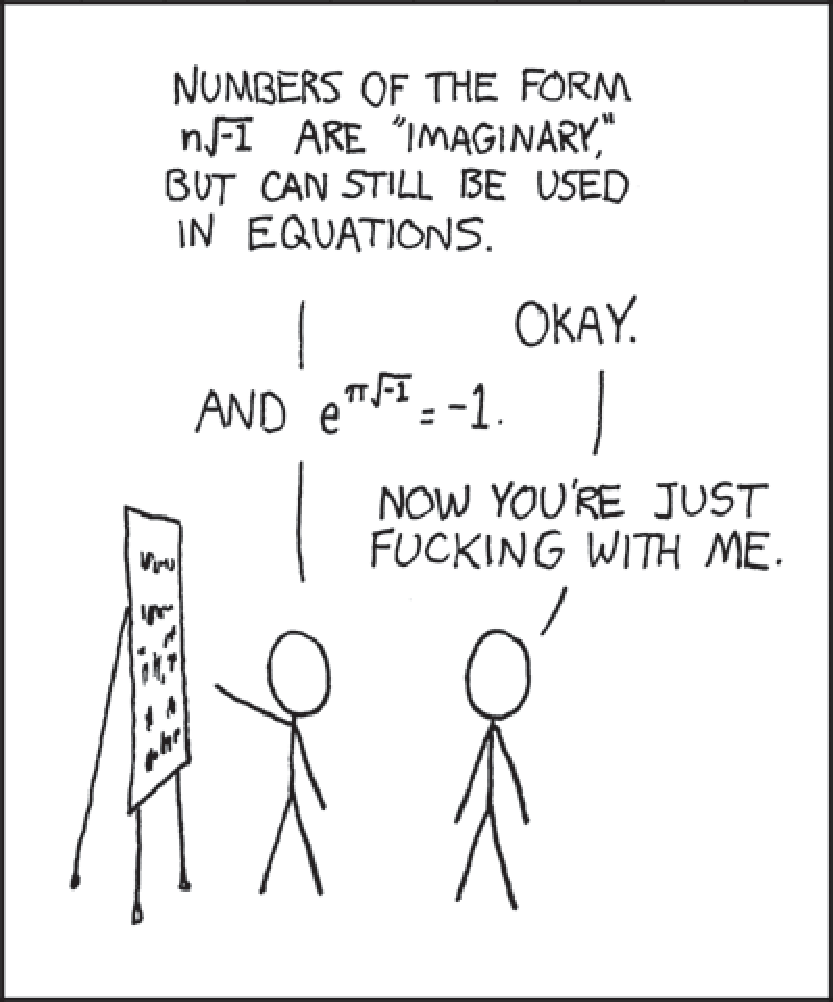
\includegraphics[width=15pc]{math_primer/figures/e_to_the_pi_times_i.eps}
  }
  \caption{$e$ to the $\pi$ times $i$.  Source: Randall Munroe,
  \protect\url{http://www.xkcd.org}.}
  \label{fig-eipi}
\end{figure}


\subsection{Algebra of Complex Numbers}

Complex numbers follow the usual algebraic rules, with the additional property
that $i^2 = -1$. For two complex numbers $z_1 = a + ib$ and $z_2 = c + id$,

\begin{align*}
    z_1 + z_2 &= (a+c) + i(b+d), \\
    z_1 z_2 &= (ac - bd) + i(ad + bc).
\end{align*}

Division is most easily performed by multiplying numerator and denominator by
the complex conjugate:
\begin{equation}
    \frac{z_1}{z_2} = \frac{z_1 z_2^*}{z_2 z_2^*}.
\end{equation}

In polar (exponential) form, multiplication and division become particularly
simple:
\begin{align}
    z_1 z_2 &= |z_1||z_2| e^{i(\theta_1 + \theta_2)}, \\
    \frac{z_1}{z_2} &= \frac{|z_1|}{|z_2|} e^{i(\theta_1 - \theta_2)}.
\end{align}


\subsection{Complex Representation of Oscillations}

Complex numbers provide a compact way to represent oscillatory behaviour. Using
Euler's identity,
\begin{equation}
    e^{i \omega t} = \cos(\omega t) + i \sin(\omega t),
\end{equation}
we can represent sinusoidal functions using complex exponentials.

In practice, we often work with expressions of the form
\begin{equation}
    z(t) = A e^{i(\omega t + \phi)},
\end{equation}
where $A$ is the amplitude, $\omega$ is angular frequency, and $\phi$ is the phase.

The physically observable quantity is typically the real part,
\begin{equation}
    \Re\left[ A e^{i(\omega t + \phi)} \right] = A \cos(\omega t + \phi).
\end{equation}

This representation greatly simplifies differentiation and integration:
\begin{align}
    \frac{d}{dt} e^{i \omega t} &= i \omega e^{i \omega t}, \\
    \int e^{i \omega t} \, dt &= \frac{1}{i\omega} e^{i \omega t}.
\end{align}


\section{Hyperbolic Functions}\label{apx:hyper}

Hyperbolic functions are closely related to trigonometric functions through
complex arguments:
\begin{align}
    \cosh z &= \cos(i z), \\
    \sinh z &= -i \sin(i z).
\end{align}

Hyperbolic functions commonly arise in problems involving exponential decay or
growth, such as diffusion and electromagnetic attenuation in conductive media.

For example, solutions of the form
\begin{equation}
    e^{-k z}
\end{equation}
can be written in terms of hyperbolic functions when boundary conditions are
applied.

As you have just seen, we have been able to relate trigonometric functions to
complex numbers.  It follows from the previous section then that we can write
the $\cos$, $\sin$, and $\tan$ as
\begin{align*}
    \cos z & = \frac{e^{i z} + e^{-i z}}{2} \\
    \sin z & = \frac{e^{i z} - e^{-i z}}{2i} \\
    \tan z & = \frac{e^{i z} - e^{-i z}}{e^{i z} + e^{-i z}}.
\end{align*}

We will now define a hyperbolic function in a very similar way as
\begin{align*}
    \cosh z & = \frac{e^{z} + e^{-z}}{2} \\
    \sinh z & = \frac{e^{z} - e^{-z}}{2} \\
    \tanh z = \frac{\sinh z}{\cosh z} & = \frac{e^{z} - e^{-z}}{e^{z} + e^{-z}},
\end{align*}
and their inverse functions as,
\begin{align*}
    \cosh^{-1} \left(\frac{e^{z} + e^{-z}}{2}\right) & = z \\
    \sinh^{-1} \left(\frac{e^{z} - e^{-z}}{2}\right) & = z \\
    \tanh^{-1} \left(\frac{e^{z} - e^{-z}}{e^{z} + e^{-z}}\right) & = z. \\
\end{align*}
